\chapter{Differential equations} \label{ch:diffeqs}
In this chapter we will solve differential equations, so let's remind ourselves what they look like. A simple \textit{first order} differential equation might look like
\begin{align*}
\frac{dy}{dx} = y.
\end{align*}
The \textit{order}, then, refers to the largest number of derivatives of $y$ in this case. This equation has analytic solution
\begin{align*}
y(x) = A e^x
\end{align*}
for arbitrary constant $A$. A second order differential equation with constant coefficients could look like
\begin{align*}
m \frac{d^2f}{dt^2} + \beta \frac{df}{dt} + k f = \cos t
\end{align*}
which has analytic solution
\begin{align*}
f(t) = A \cos \omega t +  B \sin \omega t + C \cos t
\end{align*}
for arbitrary constants $A$ and $B$, and constant $C$ as some mixture of the constants $m$, $\beta$, and $k$.

Now, these previous examples have analytic solutions because they were chosen to be simple. It turns out that most differential equations, in the sense of choosing any functions as driving terms or non-constant coefficients, do not have analytic solutions. Even an equation as simple as
\begin{align*}
\frac{dy}{dx} = x - y^2
\end{align*}
may not have an analytic solution.

In this chapter, we will restric ourselves to first order ordinary (1 variable) differential equations (ODEs) of the form
\begin{align*}
\frac{dy}{dx} = f(x,y)
\end{align*}
because many higher order ODEs cn be broken down into coupled first order ODEs, and then the techniques we learn here can be applied. In addition to the differential equation, we specify initial conditions $(x_0,y_0)$ that will constrain the solution from a family of functions down to exactly 1 function $y(x)$. Having an ODE paired with initial conditions is called an \textit{initial value problem}. We could instead constrain the solution with 2 $y$ values, $y_A$ and $y_B$, to specify a \textit{boundary value problem}, but we will not cover that here.

We introduce methods of finding the numerical approximation to the solution, in order of increasing accuracy but also increasing computational cost. These methods are the Euler method, explicit and implicit Trapezium methods, and Heun's method.


\section{Euler method}
Consider a flow field (you can imagine wind or water velocity vectors):
\begin{figure}[H]
	\begin{center}
	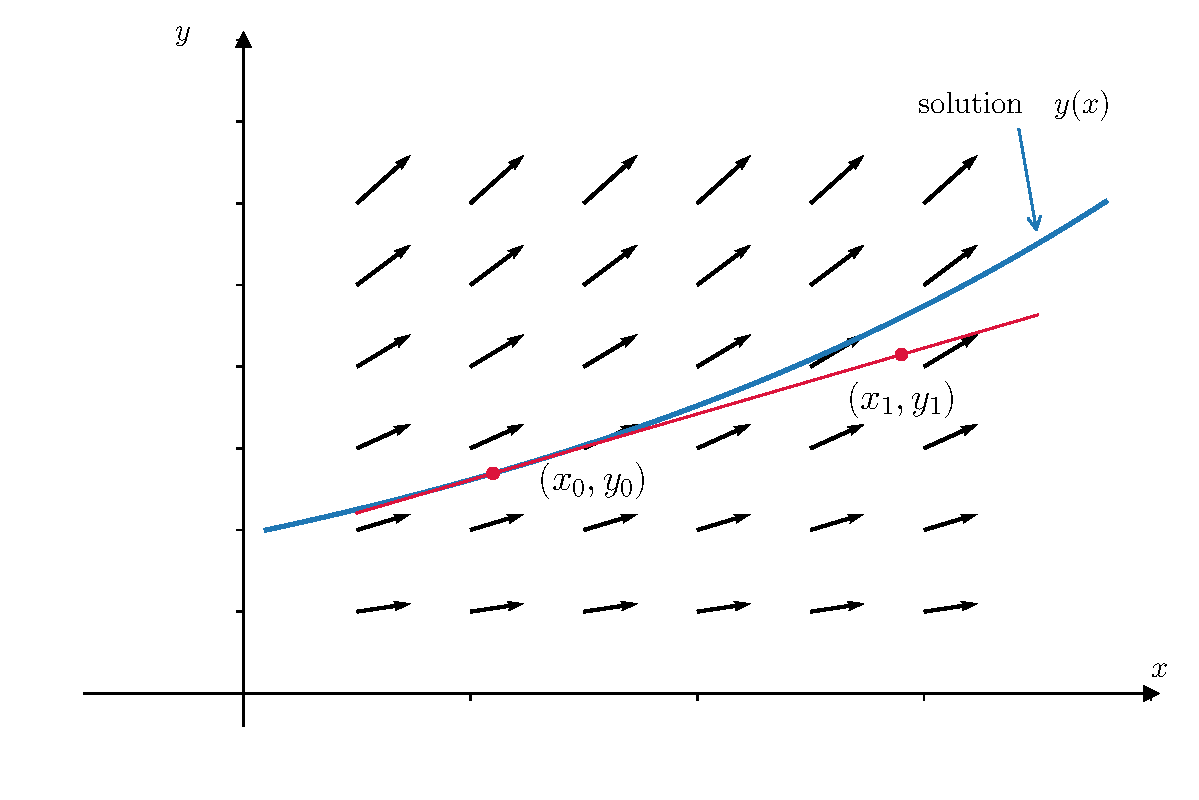
\includegraphics[width=\textwidth]{figures/ch6_idea.pdf} 
	  \caption{Vectors represent the slope function $f(x,y)$. Blue line is the true solution to the differential equation with particular initial conditions, whereas the red line is used for the Euler approximation of the next point in the numerical solution.} \label{fig:ch6_idea}
	\end{center}
\end{figure}

\noindent We want to find the path that a light ball would take if we drop it at the location $(x_0,y_0)$. At each point in space, the background velocity is given by some function
\begin{align*}
\frac{dy}{dx} = f(x,y).
\end{align*}
We can use the slope of the the solution at $(x_0,y_0)$ to estimate the next $y$ value, $y_1$, in the path after a step to $x_1$. The slope is given by the classic ``rise over run'' expression
\begin{align*}
m = \frac{y_1 - y_0}{x_1 - x_0}
\end{align*}
and we set this slope equal to the derivative at $(x_0,y_0)$
\begin{align*}
m = \frac{dy}{dx}(x_0,y_0) = f(x_0,y_0).
\end{align*}
Defining the stepsize $\Delta x = x_1 - x_0$ we then have
\begin{align*}
& \frac{y_1 - y_0}{\Delta x} = f(x_0,y_0) \\
& \implies y_1 = y_0 + \Delta x f(x_0,y_0)
\end{align*}
So we compute a new $y$ value from the old plus the derivative at the old position. This gives a general iterative scheme

\noindent \fbox{\begin{minipage}{\linewidth}
\underline{\textbf{Euler method for solving differential equations}}
\begin{align*}
y_{i+1} = y_i + \Delta x f(x_i,y_i).
\end{align*}
\end{minipage}}

This scheme is the simplest of the schemes we will look at, but it is also the least accurate.

\exemple{\upline}
{
Given the initial value problem
\begin{align*}
\frac{dy}{dx} = -y, \quad y(0)=1,
\end{align*}
compute $y(0.1)$, $y(0.2)$, and $y(0.3)$ with the Euler method with stepsize $\Delta x = 0.1$.

\noindent The Euler method equation gives
\begin{align*}
y_{i+1} &= y_i -y_i \Delta x = y_i ( 1 - \Delta x ) = 0.9 y_i.
\end{align*}
So each iteration of $y$ values is just 10\% smaller than the previous. For good measure let's compare this numerical solution with the analytic solution
\begin{align*}
y(x) = A e^{-x}.
\end{align*}
To satisfy the initial condition we must have
\begin{align*}
y(0) = A = 1.
\end{align*}
Then we tabulate the desired values, where $y_{n,i}$ is the numerical solution and $y_a(x)$ is the analytic. We will keep only 3 decimal places at each stage of the computation. This mimics the finite precision of a computer, which of course can keep many more decimal places, which is itself a source of error independent of scheme.
\begin{figure}[H]
\centering
\begin{tabular}{cccc}
$i$ & $x_i$ & $y_{n,i}$ & $y_{a}(x_i)$ \\ \hline
0 & 0   & 1     & 1 \\
1 & 0.1 & 0.900 & 0.905 \\
2 & 0.2 & 0.810 & 0.819 \\
3 & 0.3 & 0.729 & 0.741
\end{tabular}
\end{figure}

\noindent As you can see, the numerical solution is not so bad, it's correct to the first decimal place.
}{\downline}\label{ex:diff_euler}



\section{Trapezium method}
The Trapezium rule of integration (see Chapter~\ref{ch:intdiff}) will inspire a second method. Starting with the ODE
\begin{align*}
\frac{dy}{dx} = f(x,y)
\end{align*}
we integrate both sides from positions $x=x_i$ to $x=x_{i+1}$
\begin{align*}
\int_{x_i}^{x_{i+1}} \frac{dy}{dx} dx = \int_{x_i}^{x_{i+1}} f(x,y) dx.
\end{align*}
The left side can be solved with the fundamental theorem of calculus
\begin{align*}
\int_{x_i}^{x_{i+1}} \frac{dy}{dx} dx = y(x_{i+1}) - y(x_i)
\end{align*}
and the right side can be approximated with the trapezium rule
\begin{align*}
\int_{x_i}^{x_{i+1}} f(x,y) dx \sim \frac{x_{i+1} - x_{i}}{2} \left(f(x_i,y(x_i)) + f(x_{i+1},y(x_{i+1})) \right).
\end{align*}
Using the notation $y(x_k) = y_k$ and $\Delta x = x_{i+1} - x_{i}$ we have

\vspace{0.2cm}
\noindent \fbox{\begin{minipage}{\linewidth}
\underline{\textbf{Trapezium method for solving differential equations}}
\begin{align*}
y_{i+1} = y_i + \frac{\Delta x}{2} \left(f(x_i,y_i) + f(x_{i+1},y_{i+1}) \right).
\end{align*}
\end{minipage}}
\vspace{0.2cm}

\noindent Take a close look at this formula. You should be suspicious that $y_{i+1}$ appears on both sides of the equation. We do not have method for calculating $y_{i+1}$ based on previously known values. However, sometimes the function $f(x,y)$ is simple enough that with a little algebraic manipulation we can find an equation with $y_{i+1}$ equal to only previously known quantities. If we can do that, then we have developed an \textit{explicit} Trapezium scheme. Otherwise we will have to be cleverer and develop an \textit{implicit} Trapezium scheme. We'll look at an example which allows an explicit scheme before thinking about implicit schemes.

\exemple{\upline}
{
Given the initial value problem
\begin{align*}
\frac{dy}{dx} = -y, \quad y(0)=1,
\end{align*}
compute $y(0.1)$, $y(0.2)$, and $y(0.3)$ with the Trapezium method with stepsize $\Delta x=0.1$.

\noindent The Trapezium method equation gives
\begin{align*}
y_{i+1} &= y_i + \frac{\Delta x}{2} \left( -y_i - y_{i+1} \right) \\
%
y_{i+1} + \frac{\Delta x}{2} y_{i+1} &= y_i  -\frac{\Delta x}{2}  y_i  \\
%
y_{i+1} &= y_i\frac{1 - \frac{\Delta x}{2}}{1 + \frac{\Delta x}{2}}  \\
%
y_{i+1} &= \frac{0.95}{1.05} y_i.
\end{align*}
This is a simple explicit scheme! Let's tabulate the results, denoted $y_{T,i}$, comparing with the Euler solution, $y_{E,i}$, and the analytic solution, $y_{a}(x_i)$, given in the previous example. Also, let's keep 5 decimal places this time.
\begin{figure}[H]
\centering
\begin{tabular}{ccccc}
$i$ & $x_i$ & $y_{T,i}$ & $y_{E,i}$ & $y_{a}(x_i)$ \\ \hline
0 & 0   & 1       & 1     & 1         \\
1 & 0.1 & 0.90476 & 0.90000 & 0.90484 \\
2 & 0.2 & 0.81859 & 0.81000 & 0.81873 \\
3 & 0.3 & 0.74063 & 0.72900 & 0.74081
\end{tabular}
\end{figure}
We see that the Trapezium method is more accurate than Euler. It is accurate to the third decimal place in this problem.
}{\downline}

Now, if your ODE is more complicated you may not be able to make the algebraic manipulation. In this case we solve it with an implicit scheme. Define $z=y_{i+1}$ as the unknown we wish to find, while $y_i$, $\Delta x$, $x_i$ and $x_{i+1}$ are all known quantities. Then we can rearrange the Trapezium method equation to be in the form of a rootfinding problem
\begin{align*}
F_{i+1}(z) = z - y_i - \frac{\Delta x}{2} \left(f(x_i,y_i) + f(x_{i+1},y_{i+1}) \right) = 0.
\end{align*}
So the quantity we want, $y_{i+1}$, is the root of $F_{i+1}(z)=0$. This means we can use a rootfinding method (see Chapter~\ref{ch:rootfinding})! It's most common to use Newton's method here. As rootfinding methods require an initial guess, we can even use the Euler method to give a fairly good first guess $z_0 = y_i + \Delta x f(x_i,y_i)$. So, this implicit method can be summarised by the following algorithm, for solving an ODE with initial condition $y_0 = y(x_0)$:
\begin{enumerate}
	\item Choose a stepsize $\Delta x$; \\
	Suppose we've solved until $(x_i, y_i)$
	\item Use Newton's method to find root
	\begin{itemize}
		\item $F_{i+1}(z) = z - y_i - \frac{\Delta x}{2} \left(f(x_i,y_i) + f(x_{i+1},y_{i+1}) \right) = 0$
		\item $z_{k+1} = z_k - F_{i+1}(x_k)/F_{i+1}'(x_k)$ \\
		If the derivative of $F_{i+1}$ can't be analytically found, then we could estimate it as in Chapter~\ref{ch:intdiff}: e.g.,
		\begin{align*}
		F_{i+1}'(x) \sim \frac{F_{i+1}(x+\Delta x') - F_{i+1}(x\Delta x')}{2\Delta x'}
		\end{align*}
		and to be more accurate we could choose $\Delta x' < \Delta x$, for example $\Delta x' = \Delta x / 2$.
		\item Iterate Newton's method until you satisfy a pre-chosen condition, for example until the 6th decimal stops changing.
	\end{itemize}
	\item The root, $z=y_{i+1} = y(x_i + \Delta x)$;
	\item Go back to step 2 and repeat process as many times as you wish.
\end{enumerate}


\subsection{Heun's method}
Instead of relying on luck, hoping that we happen to get an explicit method, we can sacrifice some accuracy to guarantee an explicit form. In this way we also avoid the computational complexity of an \textit{implicit} scheme. Recall the Trapezium rule
\begin{align*}
y_{i+1} = y_i + \frac{\Delta x}{2} \left(f(x_i,y_i) + f(x_{i+1},y_{i+1}) \right).
\end{align*}
In Heun's method we replace the $y_{i+1}$ on the right side with an estimate $\tilde{y}_{i+1}$ given by the Euler scheme. That is,

\vspace{0.2cm}
\noindent \fbox{\begin{minipage}{\linewidth}
\underline{\textbf{Heun's method for solving differential equations}}
\begin{align*}
& y_{i+1} = y_i + \frac{\Delta x}{2} \left(f(x_i,y_i) + f(x_{i+1},\tilde{y}_{i+1}) \right), \\ 
\text{with} \quad & \tilde{y}_{i+1} = y_i + \Delta x f(x_i,y_i).
\end{align*}
\end{minipage}}
\vspace{0.2cm}

With this replacement we recover an explicit scheme, with $y_{i+1}$ equal to a collection of known terms $y_i$, $x_i$ and $\Delta x$. Let's see how this works.

\exemple{\upline}
{
Given the initial value problem
\begin{align*}
\frac{dy}{dx} = -y, \quad y(0)=1,
\end{align*}
compute $y(0.1)$, $y(0.2)$, and $y(0.3)$ with Heun's method for stepsize $\Delta x=0.1$.

\noindent Euler's method gives the first approximation of $y_{i+1}$ as calculated in example~\ref{ex:diff_euler}
\begin{align*}
\tilde{y}_{i+1} &= 0.9 y_i.
\end{align*}
This is inserted into the Trapezium rule
\begin{align*}
y_{i+1} &= y_i + \frac{\Delta x}{2} \left(f(x_i,y_i) + f(x_{i+1},\tilde{y}_{i+1}) \right) \\
%
&= y_i + \frac{0.1}{2} \left(-y_i + 0.9 y_i \right) \\
%
&= y_i + y_i  \frac{0.1}{2} \left(-0.1\right) \\
%
&= y_i - y_i 0.005 \\
%
y_{i+1}&= 0.905 y_i.
\end{align*}
There we have our simple explicit scheme. Note the previous full Trapezium rule explicit scheme in the previous example gave
\begin{align*}
y_{i+1} = \frac{0.95}{1.05} y_i \sim 0.90476 y_i
\end{align*}
which is the same if we cutoff at 3 decimal places.

Let's tabulate the results, denoted $y_{H,i}$, comparing with the Trapezium solution, $y_{T,i}$, Euler solution, $y_{E,i}$, and the analytic solution, $y_{a}(x_i)$, given in the previous examples. Also, let's keep 5 decimal places this time.
\begin{figure}[H]
\centering
\begin{tabular}{cccccc}
$i$ & $x_i$ & $y_{H,i}$ & $y_{T,i}$ & $y_{E,i}$ & $y_{a}(x_i)$ \\ \hline
0 & 0   & 1       & 1       & 1     & 1         \\
1 & 0.1 & 0.90500 & 0.90476 & 0.90000 & 0.90484 \\
2 & 0.2 & 0.81903 & 0.81859 & 0.81000 & 0.81873 \\
3 & 0.3 & 0.74122 & 0.74063 & 0.72900 & 0.74081
\end{tabular}
\end{figure}
We see that Heun's method is less accurate than the Trapezium method, but more accurate than Euler. It is accurate to the second decimal place in this problem.
}{\downline}

\section{Reduction of second order differential equations}

%\section{Runge-Kutta methods}
%Maybe next time.

\section{Summary}
We have looked at four methods for computing numerical solutions to first order differential equations, the Euler method, explicit and implicit Trapezium methods, and Heun's method. The main take away message is the balancing act of accuracy and complexity. We always pay for more accuracy with complexity. In the explicit schemes, the end results were equations that were equally easy to iterate with a computer, that is, a computer would take the same amount of time. But we paid for it with complexity in the algebraic derivation of the schemes. In the implicit scheme, the algebraic derivation is simple, but the computational power is shifted to the implementation of the root-finding algorithm, and so it will generally take a computer longer to calculate the numerical solution than with the explicit schemes. However, the implicit schemes will be more flexible in the sense of being able to work on complicated functions that don't require you to do much algebraic work (often pen and paper) before throwing the problem at the computer.






%%%%%%%%%%%%%%%%%%%%%%%%%%%%
%%%%%%%%%%%%%%%%%%%%%%%%%%%%
%%%%%%%%%%%%%%%%%%%%%%%%%%%%
%%%% Exercises %%%%
%%%%%%%%%%%%%%%%%%%%%%%%%%%%
%%%%%%%%%%%%%%%%%%%%%%%%%%%%
%%%%%%%%%%%%%%%%%%%%%%%%%%%%
\exercises{
\newpage
\section{Exercises}

\exercice{Consider $y'(x) = -2y$}
\begin{enumerate}[label=\alph*)]
	\item Write the iteration scheme given by Euler's method.
	
	\item Write the iteration scheme given by the implicit Trapezium method. Define a function $F(z)$ so that the root of the equation $F(z)=0$ is equal to the next iteration of the solution in your iteration scheme.
	
	\item From the Trapezium method, propose an explicit iteration scheme to solve the differential equation.
	
	\item Write the iteration scheme given by the second order Runge-Kutta method. 
	
	\item Write the iteration scheme given by the fourth order Runge-Kutta method.
	
	\item What is the analytic solution of the differential equation?
\end{enumerate}



\exercice{Consider $y'(x) = xy$}
\begin{enumerate}[label=\alph*)]
	\item Write the iteration scheme given by Euler's method.
	
	\item Write the iteration scheme given by the implicit Trapezium method. Define a function $F(z)$ so that the root of the equation $F(z)=0$ is equal to the next iteration of the solution in your iteration scheme.
	
	\item From the Trapezium method, propose an explicit iteration scheme to solve the differential equation.
	
	\item Write the iteration scheme given by the second order Runge-Kutta method. 
	
	\item Write the iteration scheme given by the fourth order Runge-Kutta method.
	
	\item What is the analytic solution of the differential equation?
\end{enumerate}



\exercice{Consider $y'(x) = -2y^2$}

\textit{Keep 4 decimal places throughout your calculations in the following questions.}
\begin{enumerate}[label=\alph*)]
	\item Estimate $y(0.1)$ using Euler's method, with $y(0)=2.0$ and $h=0.1$.
	
	\item Estimate $y(0.1)$ using Euler's method, with $y(0)=2.0$ and $h=0.05$.
	
	\item Estimate $y(0.1)$ using the implicit Trapezium method, with $y(0)=2.0$ and $h=0.1$. Use Newton’s method to find the root to 4 decimal places.
	
	\item Estimate $y(0.1)$ using the implicit Trapezium method, with $y(0)=2.0$ and $h=0.05$. Use Newton’s method to find the root to 4 decimal places.
	
	\item From the Trapezium method, propose an explicit method for answering the previous 2 quesitons.
	
	\item Estimate $y(0.1)$ using the second order Runge-Kutta method, with $y(0)=2.0$ and $h=0.1$.
	
	\item Estimate $y(0.1)$ using the second order Runge-Kutta method, with $y(0)=2.0$ and $h=0.05$.
	
	\item Estimate $y(0.1)$ using the fourth order Runge-Kutta method, with $y(0)=2.0$ and $h=0.1$.
	
	\item Estimate $y(0.1)$ using the fourth order Runge-Kutta method, with $y(0)=2.0$ and $h=0.05$.
	
	\item Compare your answers to the analytic solution.
\end{enumerate}



\exercice{Consider $y'(x) = y - 1$}

\textit{Keep 4 decimal places throughout your calculations in the following questions.}
\begin{enumerate}[label=\alph*)]
	\item Estimate $y(0.1)$ using Euler's method, with $y(0)=1.1$ and $h=0.05$.
	
	\item Estimate $y(0.1)$ using Euler's method, with $y(0)=0.9$ and $h=0.05$.
	
	\item Estimate $y(0.1)$ using the implicit Trapezium method, with $y(0)=1.1$ and $h=0.05$.
	
	\item Estimate $y(0.1)$ using the implicit Trapezium method, with $y(0)=0.9$ and $h=0.05$.
	
	\item From the Trapezium method, propose an explicit method for answering the previous 2 quesitons.
	
	\item Estimate $y(0.1)$ using the second order Runge-Kutta method, with $y(0)=1.1$ and $h=0.05$.
	
	\item Estimate $y(0.1)$ using the fourth order Runge-Kutta method, with $y(0)=1.1$ and $h=0.05$.
	
	\item Estimate $y(0.1)$ using the second order Runge-Kutta method, with $y(0)=0.9$ and $h=0.05$.
	
	\item Estimate $y(0.1)$ using the fourth order Runge-Kutta method, with $y(0)=0.9$ and $h=0.05$.
	
	\item Compare your answers to the analytic solution.
\end{enumerate}
}